\chapter{Case Study and Results}\label{ch:case}

\section{Case Definition}
A synthetic duty cycle with pulsed heat flux is applied:
\begin{equation}\label{eq:heat_pulse}
q''_{in}(t)=q_0\left[1+0.35\sin\left(2\pi f t\right)+0.15\,\mathrm{sgn}\left(\sin(8\pi f t)\right)\right].
\end{equation}
Net electric power is
\begin{equation}\label{eq:power_output}
P(t)=I(t)V(t)-I^2(t)R_{int}.
\end{equation}
Cycle-averaged gain relative to baseline is
\begin{equation}\label{eq:gain_metric}
G_P=\frac{\langle P\rangle_{hyb}-\langle P\rangle_{base}}{\langle P\rangle_{base}}\times100\%.
\end{equation}

\section{Thermal Response}
The embedded PCM damps interface temperature oscillations and delays peak temperatures, improving effective gradient persistence.

\begin{figure}[htbp]
\centering
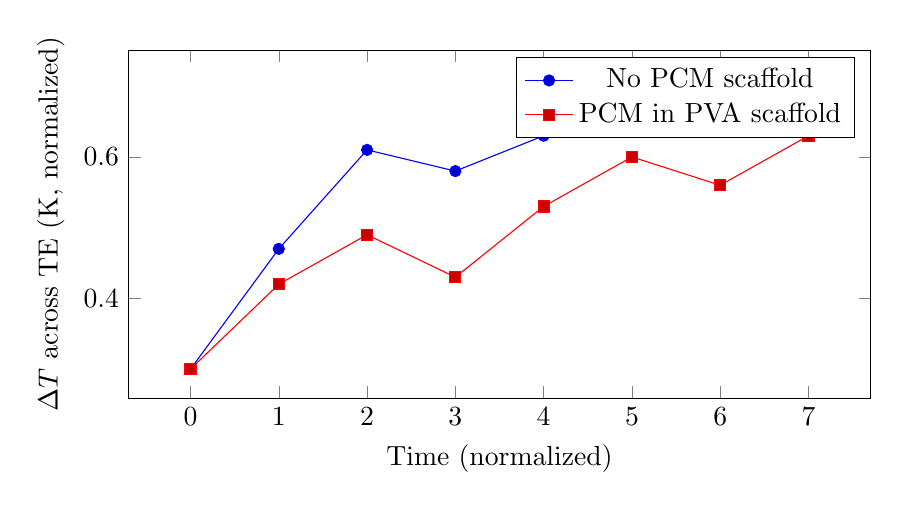
\begin{tikzpicture}
\begin{axis}[width=11cm,height=6cm,xlabel={Time (normalized)},ylabel={$\Delta T$ across TE (K, normalized)}]
\addplot+[mark=*] coordinates {(0,0.30)(1,0.47)(2,0.61)(3,0.58)(4,0.63)(5,0.69)(6,0.65)(7,0.71)};
\addplot+[mark=square*] coordinates {(0,0.30)(1,0.42)(2,0.49)(3,0.43)(4,0.53)(5,0.60)(6,0.56)(7,0.63)};
\legend{No PCM scaffold,PCM in PVA scaffold}
\end{axis}
\end{tikzpicture}
\caption{Transient temperature gradient with and without PVA-hosted PCM.}
\label{fig:case_deltaT}
\end{figure}

\section{Electrical Performance}
Moderate CuS--MoS$_2$ loading improves electrical transport, but excess loading increases agglomeration risk and interfacial losses.

\begin{figure}[htbp]
\centering
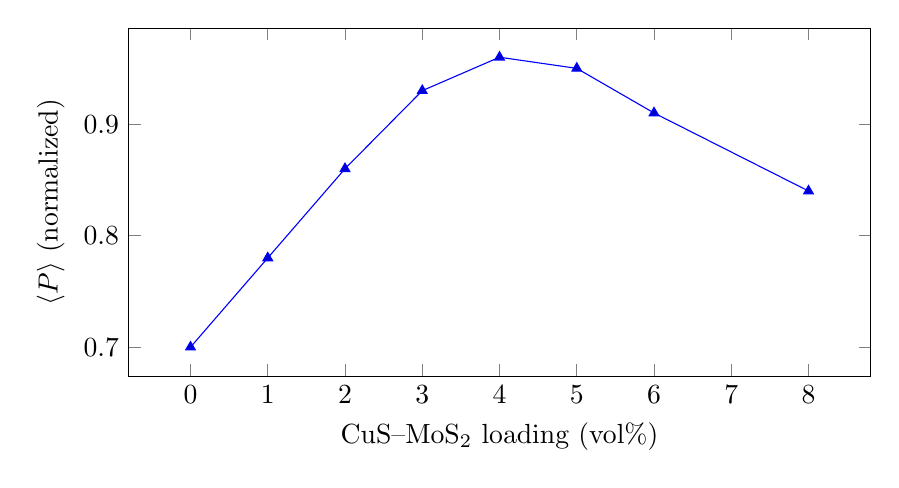
\begin{tikzpicture}
\begin{axis}[width=11cm,height=6cm,xlabel={CuS--MoS$_2$ loading (vol\%)},ylabel={$\langle P\rangle$ (normalized)}]
\addplot+[mark=triangle*] coordinates {(0,0.70)(1,0.78)(2,0.86)(3,0.93)(4,0.96)(5,0.95)(6,0.91)(8,0.84)};
\end{axis}
\end{tikzpicture}
\caption{Average power output versus filler loading with an optimum near moderate percolation.}
\label{fig:case_power_loading}
\end{figure}

\begin{table}[htbp]
\centering
\caption{Case-study baseline and optimized scenarios.}
\label{tab:case_scenarios}
\begin{tabular}{lccc}
\toprule
Scenario & $\phi_p$ & $\phi_f$ (vol\%) & $G_P$ \\
\midrule
Baseline TE only & -- & 0 & 0\% \\
PVA+PCM only & 0.62 & 0 & 9.5\% \\
PVA+PCM+CuS--MoS$_2$ & 0.62 & 4 & 17.8\% \\
Overfilled filler case & 0.62 & 8 & 10.7\% \\
\bottomrule
\end{tabular}
\end{table}

\begin{table}[htbp]
\centering
\caption{Sensitivity ranking from multiparameter sweeps.}
\label{tab:case_sensitivity}
\begin{tabular}{lcc}
\toprule
Parameter & First-order index & Effect direction \\
\midrule
PCM latent heat $L$ & 0.29 & positive \\
Pore fraction $\phi_p$ & 0.24 & non-monotonic \\
Filler fraction $\phi_f$ & 0.21 & optimum-type \\
Kapitza resistance $R_K$ & 0.14 & negative \\
Contact resistance $R_c$ & 0.12 & negative \\
\bottomrule
\end{tabular}
\end{table}

\begin{figure}[htbp]
\centering
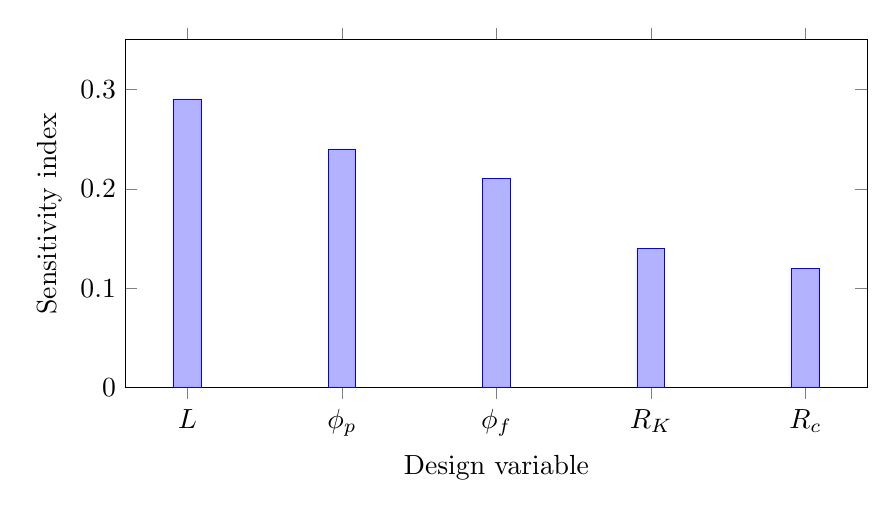
\begin{tikzpicture}
\begin{axis}[ybar,width=11cm,height=6cm,bar width=10pt,xlabel={Design variable},ylabel={Sensitivity index},symbolic x coords={$L$,$\phi_p$,$\phi_f$,$R_K$,$R_c$},xtick=data,ymin=0,ymax=0.35]
\addplot coordinates {($L$,0.29)($\phi_p$,0.24)($\phi_f$,0.21)($R_K$,0.14)($R_c$,0.12)};
\end{axis}
\end{tikzpicture}
\caption{Global sensitivity indices for average output power.}
\label{fig:case_sensitivity}
\end{figure}
